\documentclass{beamer}
%\usepackage[T1]{fontenc}
\usepackage[utf8]{inputenc}
%\usepackage{lmodern}  % Use the Latin Modern font family

\usepackage{latexsym,amsmath,xcolor,bm, amssymb, color, tikz, graphicx, amsthm, mathtools}
\usepackage{algorithm}
\usepackage{algorithmic}
\usepackage{hyperref}
\usepackage{float}     
\usepackage{CJKutf8}
\usepackage{multicol}

\DeclareMathOperator*{\argmax}{arg\,max}
\DeclareMathOperator*{\argmin}{arg\,min}
\DeclareMathOperator{\sign}{sign}
\DeclareMathOperator{\Tr}{Tr}

\makeatletter
\DeclareRobustCommand\onedot{\futurelet\@let@token\@onedot}
\def\@onedot{\ifx\@let@token.\else.\null\fi\xspace}
\def\eg{\emph{e.g}\onedot} 
\def\Eg{\emph{E.g}\onedot}
\def\ie{\emph{i.e}\onedot} 
\def\Ie{\emph{I.e}\onedot}
\def\cf{\emph{c.f}\onedot} 
\def\Cf{\emph{C.f}\onedot}
\def\etc{\emph{etc}\onedot} 
\def\vs{\emph{vs}\onedot}
\def\wrt{w.r.t\onedot} 
\def\dof{d.o.f\onedot}
\def\etal{\emph{et al}\onedot}
\makeatother


\usetheme{Madrid}
\useinnertheme{circles}


\definecolor{ColorUNR}{HTML}{0b2755} 
\usecolortheme[named=ColorUNR]{structure}
%\usecolortheme[named=ColorUNR]{exampleblock}

%\setbeamertemplate{blocks}[rounded][shadow=true]
%\setbeamercolor{block body}{fg=black,bg=white}



%------------------------------------------------------------
%This block of code defines the information to appear in the
%Title page
\title %optional
{Feedback}

\subtitle{tu opinión nos ayuda a mejorar}

%\subtitle{with applications to persuation and lie production}
% \author % (optional)
% {Author Name}

\author[Matias Ramos]{Matias Ramos}

\institute[]{Universidad Tecnológica Nacional - Facultad Regional Santa Fe}
\date[TC 2025]{Training Camp 2025}
\titlegraphic{
\includegraphics[clip,height=2cm,keepaspectratio]{logos/tcarg.jpeg}}

%End of title page configuration block
%------------------------------------------------------------


%------------------------------------------------------------
%The next block of commands puts the table of contents at the 
%beginning of each section and highlights the current section:
\AtBeginSection[]
{
  \begin{frame}
    \frametitle{Outline}
    \tableofcontents[currentsection]
  \end{frame}
}
%------------------------------------------------------------


\begin{document}


%The next statement creates the title page.
\frame{\titlepage}

% Sponsors frames (copy from template)
% --- Sponsors Frame 1: Organizador & Diamond Plus ---

\begin{frame}{Gracias Sponsors!}
    \begin{columns}[t]
        \column{0.5\textwidth}
        \centering
        Organizador\\
        \vspace{0.5cm}
        
\includegraphics[width=1\textwidth,keepaspectratio]{logos/aapc.png}
        
\includegraphics[width=1\textwidth,keepaspectratio]{logos/utn_santafe.png}
        \column{0.5\textwidth}
        \centering
        Diamond Plus\\
        
\includegraphics[width=1\textwidth,keepaspectratio]{logos/GTSlogo.jpeg}
    \end{columns}
\end{frame}

% --- Sponsors Frame 2: Gold & Oro ---

\begin{frame}{Gracias Sponsors!}
    % Platino at the top, full width
    \centering
    Platino\\
    
\includegraphics[width=0.6\textwidth,keepaspectratio]{logos/folder.png}
    
    \vfill
    
    % Gold and Oro at the bottom in two columns
    \begin{columns}[b]
        % Gold column
        \column{0.5\textwidth}
        \centering
        Gold\\
        
\includegraphics[width=0.8\textwidth,keepaspectratio]{logos/neuralsoft.png}
        % Oro column
        \column{0.5\textwidth}
            \centering
        Oro\\
        
\includegraphics[width=0.8\textwidth,keepaspectratio]{logos/jerarquicos.jpg}
    \end{columns}
\end{frame}

% --- Sponsors Frame 3: Aliado ---

\begin{frame}{Gracias Sponsors!}
    \centering
    Aliado\\
    \vspace{1cm}
    
\includegraphics[width=0.6\textwidth,keepaspectratio]{logos/santa_fe_logo_v2.jpg}
\end{frame}

% Add feedback section with QR code
\section{Momento de completar el form}

\begin{frame}{Momento de completar el form}
    \begin{center}
        
\includegraphics[width=0.5\textwidth,keepaspectratio]{img/qr-code-form-feedback.png}
    \end{center}
\end{frame}

% Add results section
\section{ahora veamos los resultados}

\begin{frame}{ahora veamos los resultados}
    \begin{center}
        \Large
        \textbf{veamos y hablemos}
    \end{center}
\end{frame}

% Feedback to participants section
\section{voy a darles feedback a ustedes}

\begin{frame}{ya estamos grandes}
    \begin{center}
        
\includegraphics[width=0.5\textwidth,keepaspectratio]{img/adult.jpeg}
    \end{center}
\end{frame}

\begin{frame}{ya estamos grandes 2}
    \begin{center}
        \begin{minipage}{0.48\textwidth}
            \centering
            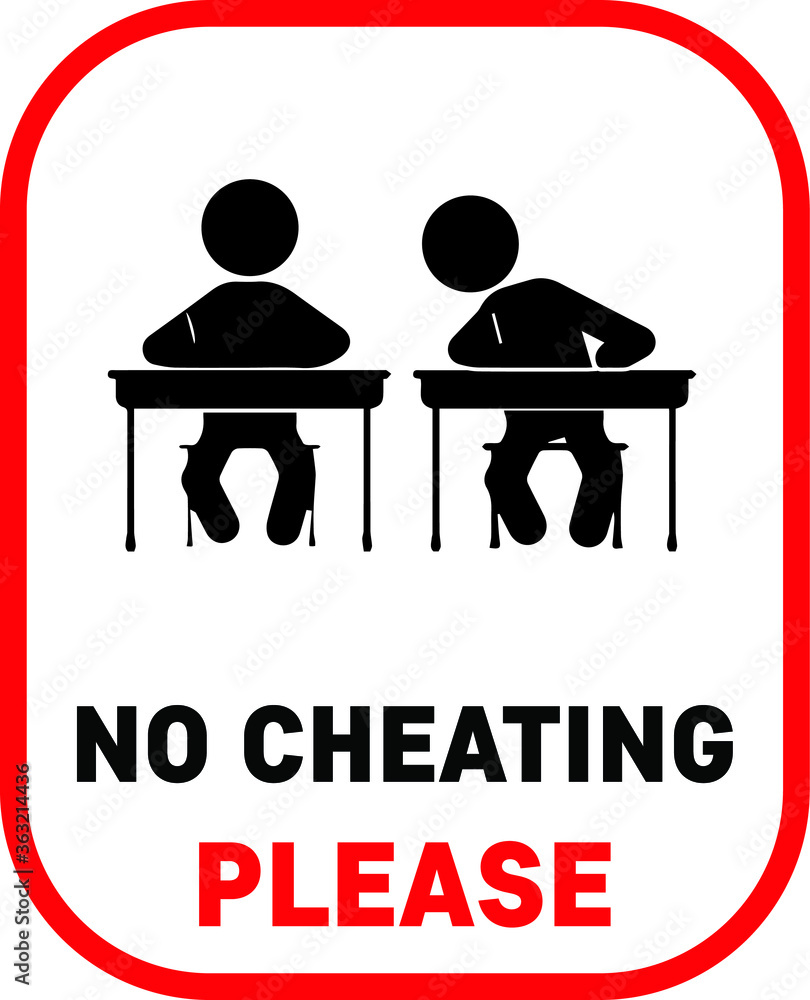
\includegraphics[width=0.95\textwidth,keepaspectratio]{img/no-cheat.jpg}
        \end{minipage}
        \hfill
        \begin{minipage}{0.48\textwidth}
            \centering
            
\includegraphics[width=0.95\textwidth,keepaspectratio]{img/do-not-use-ai.png}
        \end{minipage}
    \end{center}
\end{frame}

\end{document}